\section{Задача №2}
\textbf{Постановка задачи}:
Сформулировать и решить задачу о свободных колебаниях конечного стержня $x\in[0;l]$, $l = 0,1$м, $a^{2} = 10^{6}$ с нулевым начальным отклонением и начальной скоростью $\varphi_{2}(x) = \sin{\dfrac{\pi x}{l}}$, когда левый конец зажат, а правый движется по закону $\mu_{2} = 10^{-3}t$. Результаты $u(x, t)$ вывести графически.

\textbf{Решение}:
Сформулируем задачу:

$$
\begin{cases}
u_{tt}(x, t) = a^{2}u_{xx},&\text{$x\in[0;l]; t > 0$}\\
u(x, 0) = 0,&\text{$x\in[0;l]; t = 0$;}\\
u_{t}(x, 0) = \sin{\dfrac{\pi x}{l}},&\text{$x\in[0;l]; t = 0$;}\\
u(0, t) = 0,&\text{$x=0; t > 0$;}\\
u(l, t) = \mu_{2}(t) = 10^{-3}t,&\text{$x=l; t > 0$.}
\end{cases}
$$

Решим задачу методом редукции:

$$ u = u_{1} + u_{2}$$

$$
\begin{cases}
u_{1tt} + u_{2tt} = a^{2}(u_{1xx} + u_{2xx})\\
u_{1}(x, 0) + u_{2}(x, 0) = 0\\
u_{1t}(x, 0) + u_{2t}(x, 0) = \sin{\dfrac{\pi x}{l}}\\
u_{1}(0, t) + u_{2}(0, t) = 0\\
u_{1}(l, t) + u_{2}(l, t) = \mu_{2}(t)
\end{cases}
$$

Решим относительно $u_{1}$:
$$
\begin{cases}
u_{1tt} = 0\\
u_{1}(0, t) = 0\\
u_{1}(l, t) = \mu_{2}(t)
\end{cases}
$$

$$ u_{1} = c_{1}x + c_{2}$$
$$ u_{1}(0, t)  = c_{2} = 0 \Rightarrow u_{1}(l, t) = c_{1}l = \mu_{2} \Rightarrow c_{1} = \dfrac{\mu_{2}}{l}$$

$$ u_{1}(x, t) = \dfrac{\mu_{2}}{l} x = \dfrac{10^{-3}}{l} x \Rightarrow u_{1}(x, 0) = 0$$

$$ u_{1t} = \dfrac{10^{-3}}{l} x$$

$$ u_{1tt} = 0$$

Решим относительно $u_{2}$:
$$
\begin{cases}
u_{2tt} = a^{2} u_{2xx}\\
u_{2}(x, 0) = -u_{1}(x, 0) = 0\\
u_{2t}(x, 0) = \sin{\dfrac{\pi x}{l}} - \dfrac{10^{-3} x}{l} = \varphi(x)\\
u_{2}(0, t) = u_{2}(l, t) = 0
\end{cases}
\eqno (I)
$$

Решим данную задачу методом разделения переменных:

$$ u_{2}(x, t) = XT \eqno (1) $$

Заметим, что это задача о свободных колебаниях конечного стержня с ненулевой начальной скоростью, когда концы жёстко зажаты.

Подставим $(1)$ в систему $(I)$:
$$
\begin{cases}
XT'' = a^{2} X''T\\
X(x)T(0) = 0\\
X(x)T'(t) = \varphi(x)\\
X(0)T(t) = 0\\
X(l)T(t) = 0
\end{cases}
$$

$$ \dfrac{1}{a^{2}} \dfrac{T''}{T} = \dfrac{X''}{X} = \lambda^{2} \Rightarrow 
\begin{cases}
T'' + a^{2} \lambda^{2} T = 0 \quad \eqno (2)\\
X'' + \lambda^{2} X = 0 \quad \eqno (3)
\end{cases}
$$

Из теории известно, что $\lambda^{2} < 0$ и $T(t) \neq 0$, иначе задача бы имела одно тривиальное решение.

Сформулируем следующую краевую задачу:
$$
\begin{cases}
X'' + \lambda^{2} X = 0\\
X(0) = 0\\
X(l) = 0
\end{cases}
$$
$$ \Rightarrow X(x) = c_{1} \cos{\lambda x} + c_{2} \sin{\lambda x}$$

Подставим краевые условия и решим полученную задачу Штурма — Лиувилля:
$$ X(0) = c_{1} \cos{0} + c_{2} \sin{0} = 0 $$
$$ X(l) = c_{2} \sin{\lambda l} = 0 \Rightarrow c_{2} \neq 0 \Rightarrow \sin{\lambda l} = 0 \Rightarrow \lambda_{k} = \dfrac{\pi k}{l}$$

$\lambda_{k}$ --- собственные значения,\\
$\sin{\dfrac{\pi k}{l}} x$ --- собственные функции, \\
$X_{k}(x) = c_{k}\sin{\dfrac{\pi k}{l}} x$

Решим $(2)$:
$$ T'' + \left( \dfrac{a\pi n}{l} \right)^{2}T = 0 \Rightarrow T_{n} = A_{n} \cos{\dfrac{a\pi n}{l}}t + B_{n} \sin{\dfrac{a\pi n}{l}}t$$

$$ u_{2}(x, t) = X(x)T(t) = \sum_{n=1}^{\infty}  \left( A^{*}_{n} \cos{\dfrac{a\pi n}{l}}t + B^{*}_{n} \sin{\dfrac{a\pi n}{l}}t \right) \sin{\dfrac{\pi n}{l}}x$$

Найдём $A^{*}_{n}$ и $B^{*}_{n}$ из начальных условий:
$$ u_{2t}(x, t) = \sum_{n=1}^{\infty} \left[ -\dfrac{a\pi n}{l} A^{*}_{n} \sin{\dfrac{a\pi n}{l}}t + \dfrac{a\pi n}{l} B^{*}_{n} \cos{\dfrac{a\pi n}{l}}t \right] \sin{\dfrac{\pi n}{l}}x$$

$$ u_{2}(x, 0) = \sum_{n=1}^{\infty} A^{*}_{n} \sin{\dfrac{\pi n}{l}}x = 0 \Rightarrow A^{*}_{n} = 0 $$

$$ u_{2t}(x, 0) = \sum_{n=1}^{\infty} \dfrac{a\pi n}{l} B^{*}_{n} \sin{\dfrac{\pi n}{l}}x = \varphi(x) = \sum_{n=1}^{\infty} \varphi_{n}(x) \sin{\dfrac{\pi n}{l}}x$$
$$ \Rightarrow B^{*}_{n} = \dfrac{l}{a\pi n} \varphi_{n}(x) = \dfrac{l}{a\pi n} \dfrac{2}{l} = \int\limits_0^l \varphi(\xi) \sin{\dfrac{\pi n}{l}} \xi d\xi = \dfrac{2}{a\pi n} \int\limits_0^l \varphi(\xi) \sin{\dfrac{\pi n}{l}} \xi d\xi$$

Подставим полученные значения:
$$ u = u_{1} + u_{2}$$
$$ u_{1}(x, t) = \dfrac{t}{10^{3}l}x$$
$$ u_{2}(x, t) = \sum_{n=1}^{l} \int\limits_0^l \dfrac{2}{a\pi n} \varphi(\xi) \sin{\dfrac{\pi n}{l}} \xi d\xi \sin{\dfrac{a\pi n}{l}}t \sin{\dfrac{\pi n}{l}}x$$

\textbf{Ответ}:
$$ u = \dfrac{t}{10^{3}l}x + \sum_{n=1}^{l}  \int\limits_0^l \dfrac{2}{a\pi n} \varphi(\xi) \sin{\dfrac{\pi n}{l}} \xi d\xi \sin{\dfrac{a\pi n}{l}}t \sin{\dfrac{\pi n}{l}}x$$

$$ \varphi(x) = \sin{\dfrac{\pi}{l}}x - \dfrac{x}{l10^{3}}$$


\textbf{Проверка}:
$$ u_{t}(x, t) = u_{1t} + u_{2t} = \dfrac{x}{l10^{3}} + \sum_{n=1}^{l} \int\limits_0^l \dfrac{2}{a\pi n} \varphi(\xi) \sin{\dfrac{\pi n}{l}} \xi d\xi \cos{\dfrac{a\pi n}{l}}t \sin{\dfrac{\pi n}{l}}x = $$
$$ = \varphi_{n}(x) = \dfrac{2}{l} \int\limits_0^l \varphi(\xi) \sin{\dfrac{\pi n}{l}} \xi d\xi = \dfrac{x}{10^{3}l} + \sum_{n=1}^{\infty} \varphi_{n}(x) \cos{\dfrac{a\pi n}{l}}t \sin{\dfrac{\pi n}{l}}x$$


$$ u(x, 0) = 0 + \int\limits_0^l \sum_{n=1}^{l} \cdot \ldots = 0$$

$$ u_{t}(x, 0) = \dfrac{x}{10^{3}l} + \sum_{n=1}^{\infty} \varphi_{n}(x) \sin{\dfrac{\pi n}{l}}x = \dfrac{x}{10^{3}l} + \varphi x = \dfrac{x}{10^{3}l} + \sin{\dfrac{\pi}{l}}x - \dfrac{x}{10^{3}l = \sin{\dfrac{\pi}{l}}x}$$

$$ u(0, t) = 0 + \int\limits_0^l \sum_{n=1}^{l} \cdot \ldots = 0$$

$$ u(l, t) = \dfrac{t}{10^{3}l}l + \int\limits_0^l \sum_{n=1}^{l} \sin{\pi n} \cdot \ldots = 10^{-3}t$$

График:\\
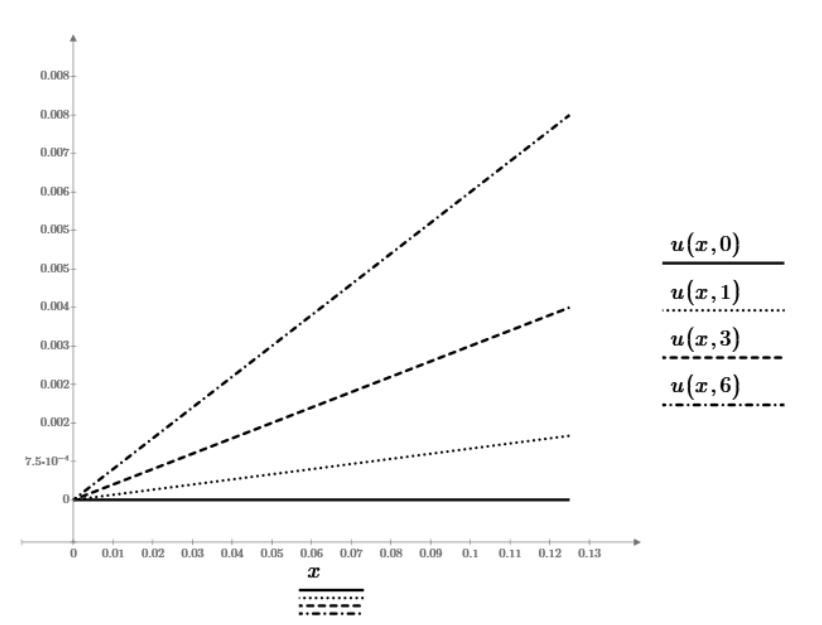
\includegraphics[width=0.8\linewidth]{2.jpg}

\pagebreak